
\bibliographystyle{plain}
\bibliography{dissertation}
\begin{document}

\chapter{Technical Background}
\label{chap:third}

For a comprehensive text analysis outcome in this study, emphasizing the context dimension is crucial for effective understanding, interpretation, and validation of results. The primary focus is on employing a text mining approach to contextualize: 1) topics derived from tax-related Twitter messages, 2) the sentiment analysis corpus, and 3) the application of machine learning prediction techniques for hashtag recommendation within the context of a tax authority. The examination of message data reveals limited use of hashtags initially in categorizing messages on Twitter, a prominent social media platform for a government department.

The rapid increase in messages, comments, and replies has surpassed the capacity for manual sorting and tagging, impeding the provision of operational services required by users. Consequently, natural language processing technology has emerged to identify pressing issues reflected by the public, prompting relevant departments to address them promptly.

\section{Research Methodology}

\subsubsection{Data}

Social media data serves as a key source of intelligence derived from the interactive dynamics between governments and citizens. The study, focusing on social media engagement for a revenue authority, specifically targeted tweets related to a tax government department in South Africa. To ensure a comprehensive representation of two-way interactions, Twitter data was exclusively collected from an account associated with the tax revenue authority. This collection comprised two distinct datasets: one encompassing government posts communicating with citizens, and the other capturing users' responses to these government tweets. The data extraction was centered around tweets containing the keyword "sarstax," a brand-established term, facilitating the identification of both the organization's messages and the corresponding engagements from citizens. Notably, despite the organization's early international inception in 2012, a significant shift in Twitter usage occurred around 2018. This approach ensures that the collected data aligns effectively with the study objectives, providing a robust foundation for analyzing social media interactions in the context of a revenue authority.

\begin{table}
\centering
\begin{tabular}{ |c|c|c|c|}
 \hline
 username & name & place &tweet\\
 language & mentions & urls & photos\\
 replies & count & retweets & count\\
 likes & count & hashtags & cashtags\\
 link & retweet & quote & url\\
 video & thumbnail & near & geo\\
 source & user rtid & user rt & retweet id\\
 reply to & retweet date\\
 \hline
 \end{tabular}
\caption{First table.}
\label{tab:table1}
\end{table}

The 2018 year marks the beginning of social media use in the revenue authority resulting in the annual data collected annually from 2018 up to year 2021. Therefore this chapter will provide a validation of two data sets that have emanated from the government tax authority usage of Twitter social media with citizens. 

\begin{itemize}
    \item Section X emanates from the brand, government tweets
    
    \item Section Y emanates from the users, citizens tweets
\end{itemize}

\subsection{Revenue Authority Tweets} 
These are tweets emanating from the revenue government for the four year period, 2018 - 2021 forming a data set of 7 877 without retweets.  However, according figure [] 13 features in the data set are not populated such as geo, quoteURL, source, near which may be important for segmentation and regional view. 

\begin{figure}[h!]
\centering
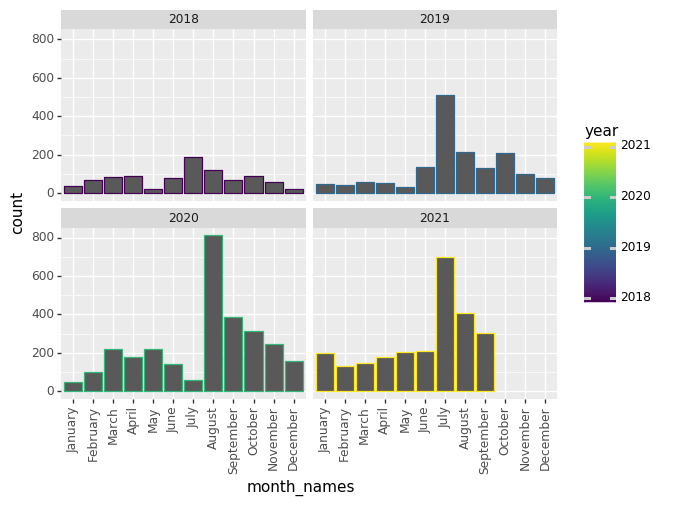
\includegraphics[width=8cm]{postgrad_template 2/Images/Gvt dataset four the four years distribution.png}
\caption{Distribution of GVT Tweets over 4 years.}
\label{fig:figure1}
\end{figure}

Within this dataset, notable aspects of tweet content include 85 percent  lacking hashtags and 26 percent devoid of user mentions. The distribution of tweets per hour reveals a spike during the morning hours, particularly between 4 am and 10 am. Regarding trigrams (3-word sequences), the most frequently repeated phrases include "check profile advice," "send details webmaster," and "send details query."

\subsection{The citizens Tweets} 

The dataset spanning four years comprises 65,919 entries and 34 features, mirroring the number of features in government tweets. Notably, approximately 80 percent of entries lack hashtags. Usernames distribution reveals 11 percent associated with government tweets, followed by 5 percent for civil societies, tax practitioners, and taxpayers each. The most frequently repeated trigrams include "judge bernard ngoepe," "illegal cigarette trade," and "illicit cigarette trade."

\subsection{Tweet Pre-Processing}
The data pre-processing stage entails removing unwanted data features that can make the data noisy for a cleaner data.  In summary the following steps were under taken:

\begin{itemize}
    \item Converting all the tweets into lower case.
\end{itemize}

\begin{itemize}
    \item removal of - duplicated tweets, punctuations, numbers (numeric data); english stop words and domain-related stop words, web links HTML tags(hyperlinks); extra blank spaces; words less than 3 characters;
\end{itemize}

\begin{itemize}
    \item Applied expansion for abbreviations; 
\end{itemize}

\begin{itemize}
    \item "The third step of pre-processing is the normalization of the text under consideration. Normalization is when all the words are brought back to their root level".
\end{itemize}

\begin{itemize}
    \item The second phase involved tokenization, to break larger chunks of data into smaller ones.
\end{itemize}

\subsubsection{Topic Modelling}

In addressing the first part of the RQ1, the age of big data applications and analytics uncovering novel data patterns, this study will employ Latent Dirichlet Allocation (LDA) Topic Model. LDA is an unsupervised machine learning approach designed to extract the meaning from large document corpora, revealing multiple patterns of topics within the text.  According to \cite{blei2011introduction}, Latent Dirichlet Allocation (LDA) is a probabilistic model aimed at uncovering concealed themes within documents, allowing for the inference of hidden topic structures. Alternatively expressed as a soft clustering algorithm, LDA is developed for various applications, including text clustering. In the context of LDA approaches, text clustering implies that each document can encompass multiple scientifically discovered topics, characterized by groups of words that frequently co-occur.
Also \cite{blei2003latent} presents LDA as a generative probabilistic model designed for collections of discrete data. It utilizes a three-level hierarchical Bayesian model to formulate topics, making it applicable to the analysis of social media data. This model illustrates the process by which a specific text corpus might have been generated from certain topics. An illustrative example is [How to identify topics in psychology using topic modeling], showcasing the application of Topic Modeling based on LDA to understand trending topics in psychology research within a large collection of documents.
\cite{mabey2018pyldavis}The exploration and presentation of discovered topics through topic models, allowing for a thorough examination of the relationships between topics and terms in an LDA model, can be facilitated by "PLDAvis," a tool accessible in Python. This tool helps address questions such as: 1) "What is the meaning of each topic?", 2) "How prevalent is each topic?", and 3) "How do the topics relate to each other?"

\subsubsection{Sentiment Analysis}

This subsection also addresses Research Question 2, which explores the evolution of computer-based sentiment analysis. Initially, sentiment analysis was limited to subjective texts available on the web and focused on online product reviews. However, post-2014, the focus shifted to social media texts, particularly from Twitter and Facebook. The significance of incorporating LDA topic modeling alongside qualitative coding for clustering is emphasized.

\cite{liu2010sentiment} describes sentiment analysis involving a series of methods, techniques, and tools for detecting and extracting subjective information, such as opinions and attitudes from language.

The outcomes of sentiment analysis/prediction encompass the labeling of each tweet/retweet based on sentiment polarity. This process enables the calculation/coding of sentiment distribution over time, providing insights into the evolving trends in citizens' behavior in response to government tweets. The final result is a visual representation of monthly sentiment trends, which assists in recognizing significant events/announcements. This strategy is enhanced by insights drawn from Topics/Wordclouds derived through topic modeling. The rationale for integrating both methods is consolidated within the Exploratory Data Analysis (EDA), while the primary focus of the methodology remains on hashtag recommendation.

\subsubsection{Hashtag Recommendation}

\cite{alsini2021hashtag} provides a review of methods for hashtag recommendation on social media platforms, specifically Twitter and Sina Weibo. The authors conduct a systematic literature review to gather research papers on this topic published between 2010 and 2020, discovering that most of the research focuses on the textual content of tweets and that collaborative filtering methods are rarely used in hashtag recommendation. Based on their findings, they propose a taxonomy of hashtag recommendation methods, including text-based methods, hybrid user-based methods, and hybrid miscellaneous methods. They also discuss the challenges and future research directions in this field.

\cite{zhao2016personalized} The paper presents a personalized hashtag recommendation approach using a Latent Dirichlet Allocation (LDA)-based topic model in a microblog environment. The approach combines user profile-based collaborative filtering and LDA-based collaborative filtering to find relevant hashtags for users. The proposed LDA-based model, called Hashtag-LDA, jointly models the relationships between users, hashtags, and words in microblogs. The experimental results on a real Twitter dataset show that the proposed recommendation approach outperforms other related methods and that Hashtag-LDA is effective in finding relevant hashtags.

\cite{godin2013using} this paper introduces an unsupervised and content-based hashtag recommendation method for tweets. The approach utilizes Latent Dirichlet Allocation (LDA) to model the underlying topic assignment of language-classified tweets. The key advantage lies in using a topic distribution for recommending general hashtags. The paper covers related work, details the process of creating a tweet dataset, and outlines the binary classification algorithm used to classify tweets as English or non-English language. The conclusion includes evaluation results and outlines future work. The content-based method employs Latent Dirichlet Allocation (LDA), a hidden generative topic model, enhancing effective categorization and search of tweets while mitigating sparse and noisy tweet content.

\cite{mehrotra2013improving} at the same time addresses challenges in applying topic models, particularly Latent Dirichlet Allocation (LDA), to Twitter content due to the concise and unstructured nature of tweets. The paper investigates various pooling schemes, emphasizing tweet pooling by hashtags, to enhance the quality of topics derived from Twitter data. Through empirical evidence, the authors show that hashtag-based pooling significantly improves topic coherence compared to other schemes and the baseline LDA model. Additionally, the automatic labeling of hashtags further enhances topic quality. The paper offers valuable insights and methods for improving LDA topic models when applied to Twitter content.

This PDF discusses the development of an interactive hashtag recommendation system for social media platforms like Twitter. The system aims to help users enhance their tweets by suggesting relevant hashtags. The system consists of two phases: divergence and convergence. In the divergence phase, the system provides users with related topics based on their input tweet, allowing them to explore novel hashtags. In the convergence phase, the system recommends more accurate hashtags based on the selected topic. The system utilizes natural language processing, topic modeling, and recommendation algorithms to achieve accurate and efficient hashtag recommendations. The system's effectiveness and usability were evaluated through user experiments, with positive results indicating that the interactive hashtag recommendation system provides accurate and helpful hashtags for users.

\cite{alsini2021hashtag} brings a discussion n the development of an interactive hashtag recommendation system for social media platforms like Twitter. The system aims to help users enhance their tweets by suggesting relevant hashtags. The system consists of two phases: divergence and convergence. In the divergence phase, the system provides users with related topics based on their input tweet, allowing them to explore novel hashtags. In the convergence phase, the system recommends more accurate hashtags based on the selected topic. The system utilizes natural language processing, topic modeling, and recommendation algorithms to achieve accurate and efficient hashtag recommendations. The system's effectiveness and usability were evaluated through user experiments, with positive results indicating that the interactive hashtag recommendation system provides accurate and helpful hashtags for users.

\cite{altinel2018semantic} discusses the topic of semantic text classification, which is the task of organizing documents into pre-determined classes using machine learning algorithms. It highlights the importance of capturing the semantics of words and the semantic connections between words, documents, and classes in order to achieve better classification performance. The PDF reviews knowledge-based approaches, such as the use of WordNet, Wiktionary, and Wikipedia as domain knowledge sources, and discusses their advantages over traditional text classification methods. It also explores corpus-based approaches that utilize statistical analysis to discover hidden connections between words in training documents. Additionally, the PDF covers deep learning-based approaches, methods that enhance word/character sequences, and linguistic enriched approaches for semantic text classification. The performance comparison of these approaches is discussed, along with their experimental results and advantages / disadvantages. Overall, the PDF provides a comprehensive overview of semantic text classification and the various approaches used in the field.

Inspired by Community question answering websites that have used both questions text or tags (keywords related to the asked question) topic modelling can summarize and describe content of the question, in this case the extension to understand the context of the tweet for themes and topics of discussion.

\cite{prabha2023question} conducted a study to support that using a text for topic modelling is producing better performance as opposed to using tags when evaluated model using tw metrics namely coherence and perplexity.  In using the users data  (tweets/text), one can determine the hidden information about the user and trending topics across domains.  Hashtags and tags provide context regarding context and semantics.

1. Data Preprocessing:
   - Tokenize the tweets: Split each tweet into individual words or tokens.
   - Remove stop words: Remove common words like "the," "is," "and," etc., as they don't contribute much to the hashtag recommendation process.
   - Stemming/Lemmatization: Reduce words to their base or root form (e.g., "running" becomes "run").
   - Vectorization: Convert the preprocessed tweets into numerical feature vectors using techniques such as TF-IDF.

2. Supervised Model Training:
   - Random Forest Classifier (RFC): Train an RFC model using the preprocessed tweet vectors and their corresponding hashtags as labels.
   - Support Vector Classifier (SVC): Train an SVC model using the same preprocessed tweet vectors and hashtag labels.

3. Unsupervised Topic Model Training:
   - Latent Dirichlet Allocation (LDA): Apply LDA to the preprocessed tweet vectors to discover latent topics within the tweet corpus.

4. Hashtag Recommendation:
   - Given a new tweet, pre-process it and convert it into a feature vector.
   - Use the trained RFC and SVC models to predict the most relevant hashtags for the tweet.
   - Utilize the LDA model to identify the latent topics in the tweet and suggest hashtags related to those topics.
   - The model only Utilized the 7887 tweet messages with identifiable hashtags
This has resulted to recommendation of topics of tweets to organise with an appropriate hashtag for improved user experience that can lead to an efficient two-way communication resulting in organization better services through continuous evidence-based decision making efforts.

\subsubsection{Model Evaluation}

[EVALUATION technique METRIC FOR HASHTAG RECOMMENDATION] The paper examines the assessment of metrics for hashtag recommendation systems, which automatically suggest hashtags to users while composing a tweet. The authors contend that widely used metrics such as hit rate, precision, recall, and F1-score may be insufficient for evaluating hashtag recommendation systems, particularly when the number of ground truth hashtags in tweets varies greatly. They introduce a novel metric termed "hit ratio" to address this issue, considering the varying number of hashtags in the recommended and ground truth sets. The hit ratio is computed as the ratio of matching hashtags over the minimum value between the number of recommended hashtags and the number of ground truth hashtags. The authors compare the hit ratio with traditional evaluation metrics, illustrating its utility through hypothetical scenarios and real-world applications. They assert that the hit ratio offers a more meaningful metric than traditional measures for the evaluation of hashtag recommendation systems.

Some of the evaluation metrics which can be used both for supervised and unsupervised techniques:

\begin{itemize}
    \item Jaccard Score: Calculates the Jaccard similarity score between the predicted hashtags and the actual hashtags for a set of test tweets. Jaccard score measures the similarity between two sets of hashtags.\\
\end{itemize}
\begin{itemize}
    \item Dummy Classifier: Build a dummy classifier to predict whether a tweet is  using the pre-processed tweet vectors for an appropriate hashtag.
\end{itemize}

\begin{itemize}
    \item to iterate and fine-tune the models and evaluation metrics based on the specific characteristics of your tweet dataset and the desired performance.
\end{itemize}
\begin{itemize}
    \item In order to evaluate the text classification supervised models in Topic Modelling unsupervised method to determine their effectiveness in analyzing short text data.   The topic modelling evaluation method is based on "the understandability of extracted topics (topic quality) besides the topic performance and accuracy by applying common standard metrics that apply to the TM domain such as recall, precision, F-score, and topic coherence".
\end{itemize}


\subsubsection{Conclusion}

In conclusion the research methodology has emphasized the importance of understanding the context and domain-specific requirements when selecting and evaluating the algorithms for hashtag recommendation. By considering the unique characteristics of Twitter or the government department's data collection efforts, the researcher has streamlined the methodology to suit the specific needs and challenges of the government environment.
In summary, the research methodology presented in this chapter provides a robust framework for text mining and production techniques aimed at recommending hashtag tags. By combining supervised and unsupervised algorithms, we have demonstrated the potential for enhancing the accuracy and efficiency of hashtag recommendation processes for Twitter or a government department involved in data collection and analysis. This methodology serves as a foundation for the subsequent stages of our research, enabling us to delve deeper into the implementation and evaluation of these techniques and ultimately contribute to the advancements in the field of text mining and recommendation systems."

\bibliographystyle{plain}
\bibliography{dissertation}

\end{document}






